\documentclass[twoside]{article}

\usepackage{lipsum} % Package to generate dummy text throughout this template
\usepackage{bm}
\usepackage{tabularx}
\usepackage{etoolbox}
\apptocmd\normalsize{%
 \abovedisplayskip=12pt plus 3pt minus 9pt
 \abovedisplayshortskip=0pt plus 3pt
 \belowdisplayskip=12pt plus 3pt minus 9pt
 \belowdisplayshortskip=7pt plus 3pt minus 4pt
}{}{}
\usepackage[utf8]{inputenc}

\usepackage[sc]{mathpazo} % Use the Palatino font
\usepackage[T1]{fontenc} % Use 8-bit encoding that has 256 glyphs
\linespread{1.05} % Line spacing - Palatino needs more space between lines
\usepackage{microtype} % Slightly tweak font spacing for aesthetics
\usepackage{floatrow}
\usepackage{verbatimbox}
\usepackage[hmarginratio=1:1,top=32mm,columnsep=20pt, outer=1.5cm]{geometry} % Document margins
\usepackage{multicol} % Used for the two-column layout of the document
\usepackage[hang, small,labelfont=bf,up,textfont=it,up]{caption} % Custom captions under/above floats in tables or figures
\usepackage{booktabs} % Horizontal rules in tables
\usepackage{float} % Required for tables and figures in the multi-column environment - they need to be placed in specific locations with the [H] (e.g. \begin{table}[H])
\usepackage{hyperref} % For hyperlinks in the PDF
\usepackage{amsmath,amssymb}
\usepackage{graphicx}
\usepackage{lettrine} % The lettrine is the first enlarged letter at the beginning of the text
\usepackage{paralist} % Used for the compactitem environment which makes bullet points with less space between them
\usepackage{subcaption}
\usepackage{appendix}


\usepackage{abstract} % Allows abstract customization
\renewcommand{\abstractnamefont}{\normalfont\bfseries} % Set the "Abstract" text to bold
\renewcommand{\abstracttextfont}{\normalfont\small\itshape} % Set the abstract itself to small italic text

\usepackage{titlesec} % Allows customization of titles
\renewcommand\thesection{\Roman{section}} % Roman numerals for the sections
\renewcommand\thesubsection{\Roman{subsection}} % Roman numerals for subsections
\titleformat{\section}[block]{\large\scshape\centering}{\thesection.}{1em}{} % Change the look of the section titles
\titleformat{\subsection}[block]{\large}{\thesubsection.}{1em}{} % Change the look of the section titles
\newcommand{\bigO}[1]{\ensuremath{\mathop{}\mathopen{}\mathcal{O}\mathopen{}\left(#1\right)}}
\def\mean#1{\left< #1 \right>}

%----------------------------------------------------------------------------------------
%	TITLE SECTION
%----------------------------------------------------------------------------------------

\title{\vspace{-15mm}\fontsize{24pt}{10pt}\selectfont\textbf{Monte Carlo Simulation of 2D Ising Model}} % Article title

\author{
\large
\textsc{Andr\'e Melo 4519302}\\
\textsc{Matteo Domenighini 4512154} \\[2mm] % Your name
\normalsize Delft University of Technology\\ % Your institution
\vspace{-5mm}
}
\date{}

%----------------------------------------------------------------------------------------

\begin{document}

\maketitle % Insert title

%----------------------------------------------------------------------------------------
%	ABSTRACT
%----------------------------------------------------------------------------------------

\begin{abstract}

\noindent The aim of this report is to present the results obtained using Monte Carlo simulation for the Ising model and XY model. Two main algorithms have been implemented to simulate the behaviour of the system: the Metropolis Monte Carlo algorithm and the Hoshen-Kopelman cluster finding algorithm. Both algorithms have been used to extrapolate relevant physical quantities, such as the magnetization, the magnetic susceptibility and the specific heat. Finite-size scaling has also been used in order to calculate the critical exponents. Using the Metropolis algorithm we were able to prove the universality of the critical exponents of the Ising model. 
The Hoshen-Kopelman algorithm is also successfully implemented for the calculation of the helicity modulus.

\end{abstract}

%----------------------------------------------------------------------------------------
%	ARTICLE CONTENTS
%----------------------------------------------------------------------------------------

\begin{multicols}{2} % Two-column layout throughout the main article text

\section{Introduction}
In this report we aim to investigate the physics of the Ising and XY models through the implementation of Monte Carlo algorithms.
The Monte Carlo algorithms are a class of algorithms in which "random" numbers play an essential role ~\cite{thijssen}. This method has been widely and successfully implemented in the past decades to simulate the behaviour of physical systems in order to extrapolate information regarding their static properties. \\
The Hoshen Kopelman algorithm is a cluster finding algorithm that has been implemented as a non-recursive alternative to the Swendsen-Wang algorithm. It is based on the more famous Union-Find algorithm.

In section II the interaction model and the working principles of the two algorithms are outlined. In section III we reported the numerical results obtained for specific heat, magnetization, magnetic susceptibility, Binder cumulant, finite-size scaling and XY Model.

%------------------------------------------------
\begin{figure*}[b]
  \begin{subfigure}[b]{0.35\textwidth}
    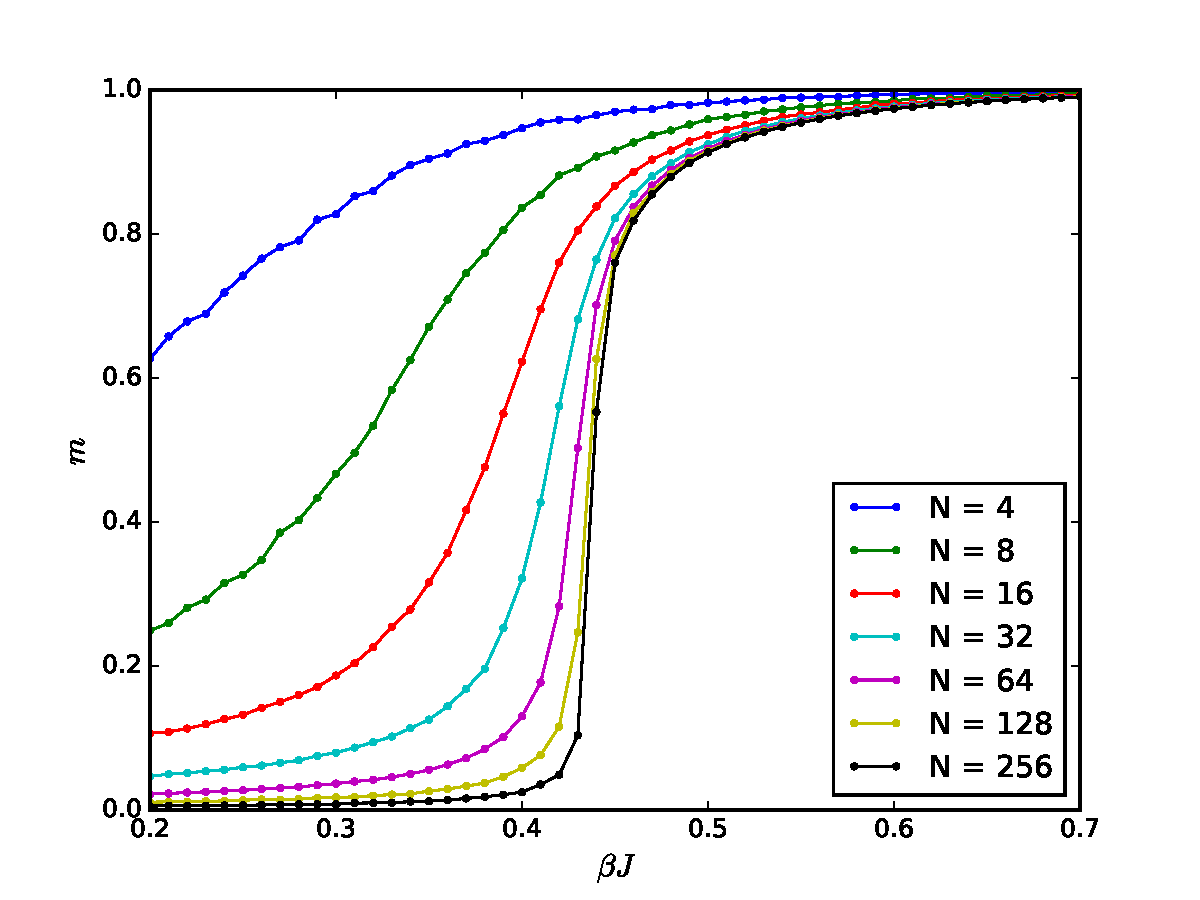
\includegraphics[width=\textwidth]{images/magnetization.pdf}
    \caption{Magnetization}
    \label{magnetization}
  \end{subfigure}
  \begin{subfigure}[b]{0.35\textwidth}
    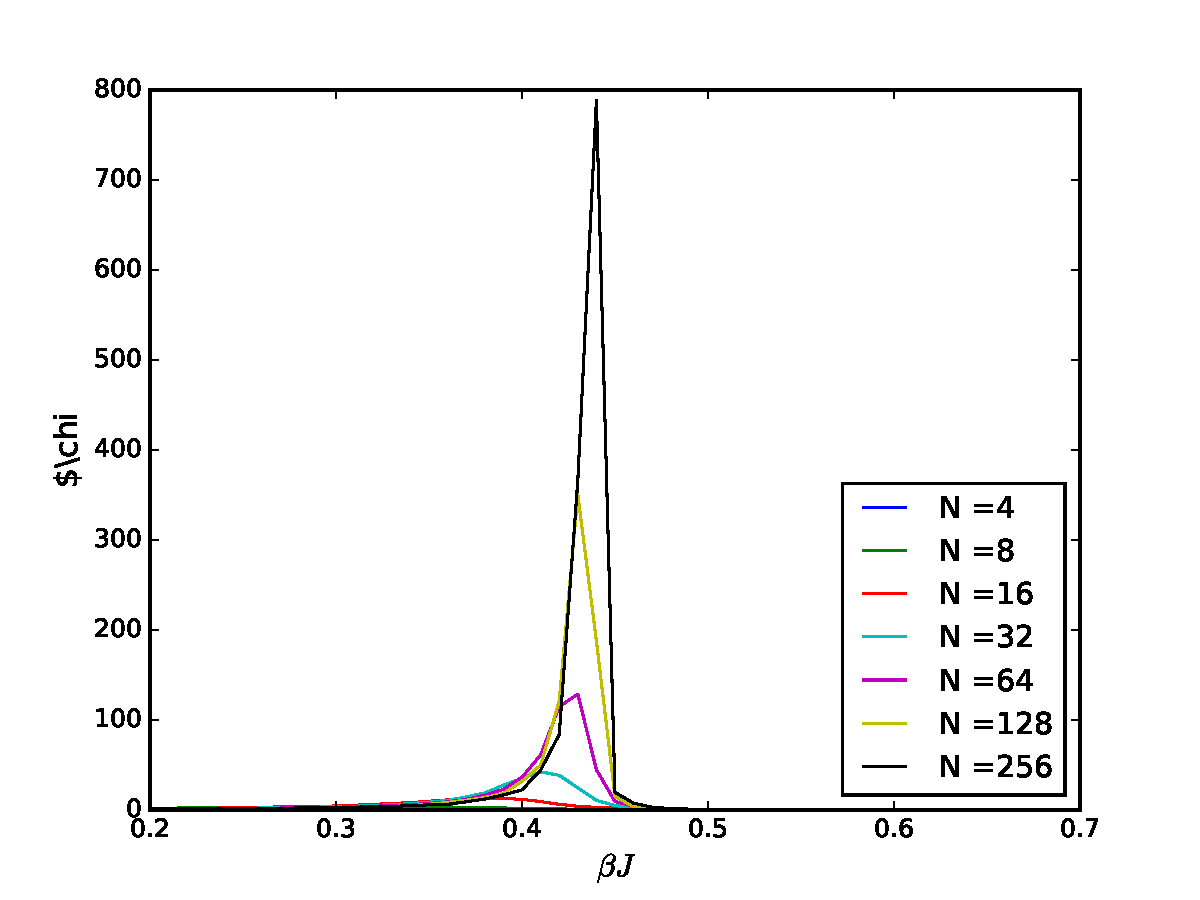
\includegraphics[width=\textwidth]{images/susceptibility.pdf}
    \caption{Susceptibility}
    \label{susceptibility}
  \end{subfigure}
  \caption{Behaviour of the magnetization and susceptibility calculated with the Hoshen-Kopelman algorithm}
\end{figure*}


\section{Methods}
While implementing the models and algorithm outlined in this section, we have considered $k_B = 1$, $J = 1$ and a unitary distance between the lattice sites.

\subsection{Ising Model}
The Ising Model describes the dynamics of a $L \times L$ lattice of spins which can take values of $\pm 1$. The Hamiltonian of the system in absence of an external magnetic field is described by

\begin{equation}
\label{ising_hamiltonian}
H = - J \sum_{\mean{ij}} s_i s_j
\end{equation}

where $s_i$ represents the spin associated with the \emph{i}th site.
When $J$ is taken to be larger than zero the system favours parallel alignment of adjacent spins (ferromagnetic behaviour). For $J<0$ anti-parallel alignment is preferable (antiferromagnetic behaviour).

The partition function for the system is given by 

\begin{equation}
\mathcal{Z} = \sum_{s_i} e^{-\beta H\left(s_i\right)}
\end{equation}

which is dependent on the temperature of the system, contained in $\beta$. 

\subsection{XY Model}
The XY Model is a generalization of the Ising model in which the spins can take on any direction in the 2D plane. The Hamiltonian for this model in the absence of a magnetic field can be written as:

\begin{equation}
H = -J \sum_{\mean{ij}} \cos(\theta_i - \theta_j)
\end{equation}

where $\theta_i$ is the angle between the direction of the spin of the \emph{i}-th site and an arbitrarily chosen axis. \\
The XY model behaviour has been simulated through a Monte Carlo simulation using the Hoshen-Kopelman algorithm, which is described in part ~\ref{hk_al} of this section.

\subsection{Metropolis Monte Carlo Algorithm}
The Metropolis Monte Carlo algorithm is an algorithm in which the information regarding different distributions of a system is stored in a Markov chain. 
In an uncorrelated chain, the probability of occurrence of a certain event is given by the product of the single probabilities lead up to the event itself. In a Markov chain, the probability of occurrence for a sequence of events is defined by the transition probability from one event (in this case, configuration) to another.
The Metropolis Monte Carlo method utilizes a Markov chain of configurations based on a given stationary distribution, which in our case is represented by the Boltzmann distribution. In order to ensure a correct representation of the phase space, the Markov chain has to be ergodic, which means that the probability of occurrence of a certain configuration has to be independent of the time $t$ when $t$ is large. \\
Considering the probability of transition between two generic states leads to the \emph{detailed balance solution}

\begin{equation}
T(X \rightarrow X') = \omega_{XX'}A_{XX'}
\end{equation}

where \textbf{$\omega$} is a symmetric matrix and represent the trial step probability, while $A_{XX'}$ represents the acceptance probability. \\
In the simulation of the Ising model with the Metropolis Algorithm, 

\begin{align}
\omega_{XX'} = \frac{1}{L^2} \qquad \text{if X and X' differ by one spin} \\
\omega_{XX'} = 0 \qquad  \text{otherwise} 
\end{align}

A spin, or more than one, are then selected at random and flipped. The difference in energy between the two configurations is then calculated. if the results is bigger than zero, the new configuration is accepted with probability $e^{-\beta\Delta E}$, while if $\Delta E < 0$, the new state is always adopted.

\subsection{Hoshen-Kopelman Algorithm} \label{hk_al}
Before applying the Hoshen-Kopelman algorithm it is necessary to find the links between lattice sites. For each link, we consider two possible cases; in the first one, the spins are opposite and the interaction is deleted; if the spins are equal the interaction is deleted with probability $e^{2\beta J}$ and frozen with probability $1-e^{-2\beta J}$.
In the simulation, determining whether a link is frozen or not implies generating a "random" number, which means that the overall algorithm still belongs to the Monte Carlo family. 

Once the links are found, one can apply the Hoshen-Kopelman cluster finding algorithm, which can be divided in two steps.
The first one consists in checking the links to the left and upwards for each site of the lattice. If there is a link between two sites, they are assigned to the same cluster. The second step consists in going over all the sites once more and checking all their links to make sure that the clusters have been correctly identified~\cite{joas}. \\ To generate random configurations, a new random spin value is then assigned to each cluster and the properties of the specific configuration are calculated.

\subsubsection{Applying the HK algorithm to XY model}
(to be written)
%------------------------------------------------

\section{Results}

\begin{figure*}[!tpb] 
 \begin{subfigure}[b]{0.35\textwidth}
    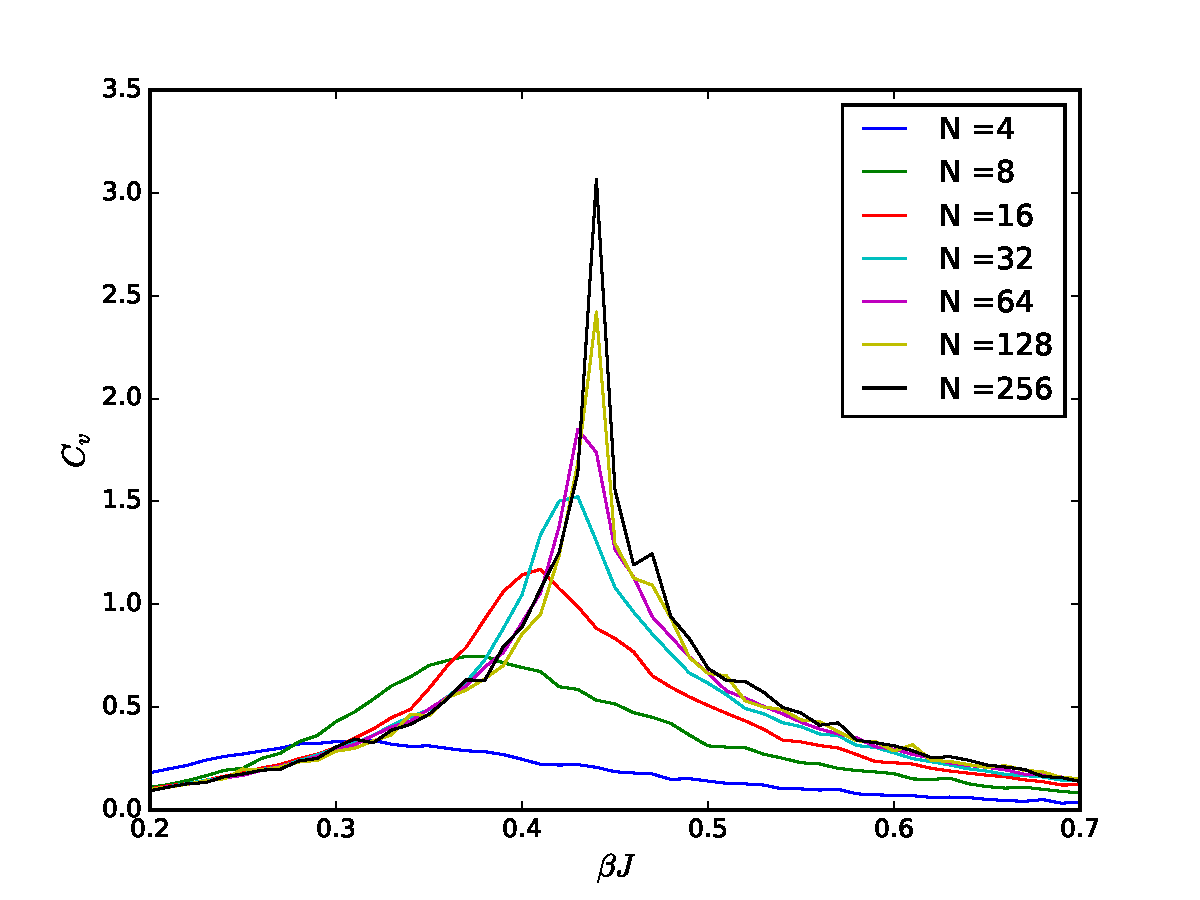
\includegraphics[width=\textwidth]{images/cv.pdf}
    \caption{Specific Heat}
    \label{cv}
  \end{subfigure}
  \begin{subfigure}[b]{0.35\textwidth}
    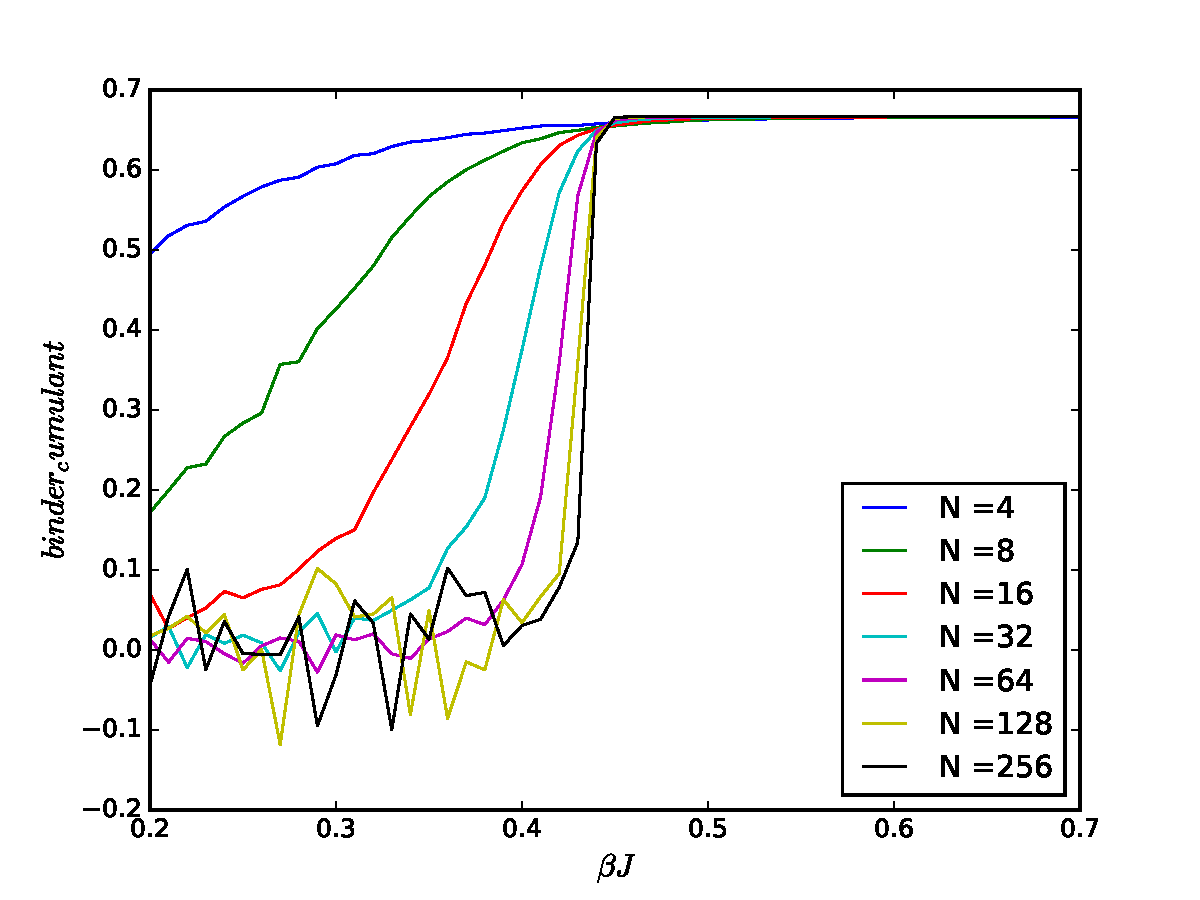
\includegraphics[width=\textwidth]{images/binder_cumulant.pdf}
    \caption{Binder cumulant}
    \label{bc}
  \end{subfigure}
  \caption{Behaviour of the specific heat and Binder cumulant calculated with the Hoshen-Kopelman algorithm}
\end{figure*}

The results obtained with the Hoshen-Kopelman algorithm for magnetization, susceptibility specific heat and Binder cumulant are presented in the first four parts of this section.
In section V we present the results obtained with finite-size scaling when also considering second neighbours with both ferromagnetic and anti-ferromagnetic behaviour. In order to consider higher interaction order, the Metropolis algorithm as been used.
In section VI we reported the results obtained for the XY model through the Hoshen-Kopelman algorithm.

It should be noted that we follow the convention found in ~\cite{thijssen}, where $k_B = 1$ and the distance between sites is taken to be unitary. The closed neighbout interactions in the simulated Ising model are ferromagnetic, which means that $J > 0$.

\subsection{Magnetization}
In the Ising model the magnetization is defined as:

\begin{equation}
m = \frac{1}{L^2} \mean{\sum_i s_i}
\label{magnetization_conventional}
\end{equation}

The spin flipping operations taking place in the Hoshen-Kopelman algorithm cause this quantity to oscillate considerably; for this reason, the magnetization can be better described as:

\begin{equation}
m = \frac{1}{L^2} \mean{\left|\sum_i s_i\right|}
\end{equation}

In Figure~\ref{magnetization} it is possible to see the behaviour of the magnetization as a function of temperature. We can clearly see a phase transition around $\beta J = 0.44$, as predicted by the theory. The exact value found for the critical point is reported in section III.V.

\subsection{Susceptibility}
The susceptibility is defined as 

\begin{equation}
\chi = \frac{dm}{dh}
\end{equation}

This definition is modified in order to account for the cluster spin flips taking place in the Hoshen-Kopelman algorithm. The resulting equation is:

\begin{equation}
\chi = \frac{1}{L^2}\left[\mean{\left(\sum_i s_i\right)^2} - \mean{\left|\sum_i s_i \right|}^2\right]
\end{equation}

The results obtained for the susceptibility are shown in Figure~\ref{susceptibility}. As expected, the susceptibility presents a peak close to the phase transition and is equal to zero everywhere else.

\subsection{Heat capacity}
The heat capacity can be directly related to the system's energy fluctuations. From \cite{thijssen}:

\begin{equation}
C_v = \frac{\mean{E^2} - \mean{E}^2}{L^2 T}
\end{equation}

The obtained results are show in Figure~\ref{cv}.

\subsection{Binder cumulant}
The Binder cumulant $Q$ is defined as:

\begin{equation}
Q = 1 - \frac{\mean{\left( \sum_i s_i \right)^4}}{3 \mean{\left( \sum_i s_i \right)^2}^2}
\end{equation}

The behaviour of the Binder cumulant is shown in Figure~\ref{bc}. It can be shown that $Q$ has a universal value at the critical point \cite{lecture_notes}. Therefore one can estimate $\beta J_c$ by determining the intersection point of $Q$ for different lattice sizes. Since intersection point is depends very weakly on the lattice size, one can an accurate estimate for critical point by interpolating the curves for the highest values of $N$ and determining the intersection. This procedures yields $\beta J_c \approx 0.4409$, which is very close to the exact value of $\beta J_c = 0.44068...$.

\subsection{Finite size scaling}
\begin{figure*}[!tpb]
  \begin{subfigure}[b]{0.32\textwidth}
    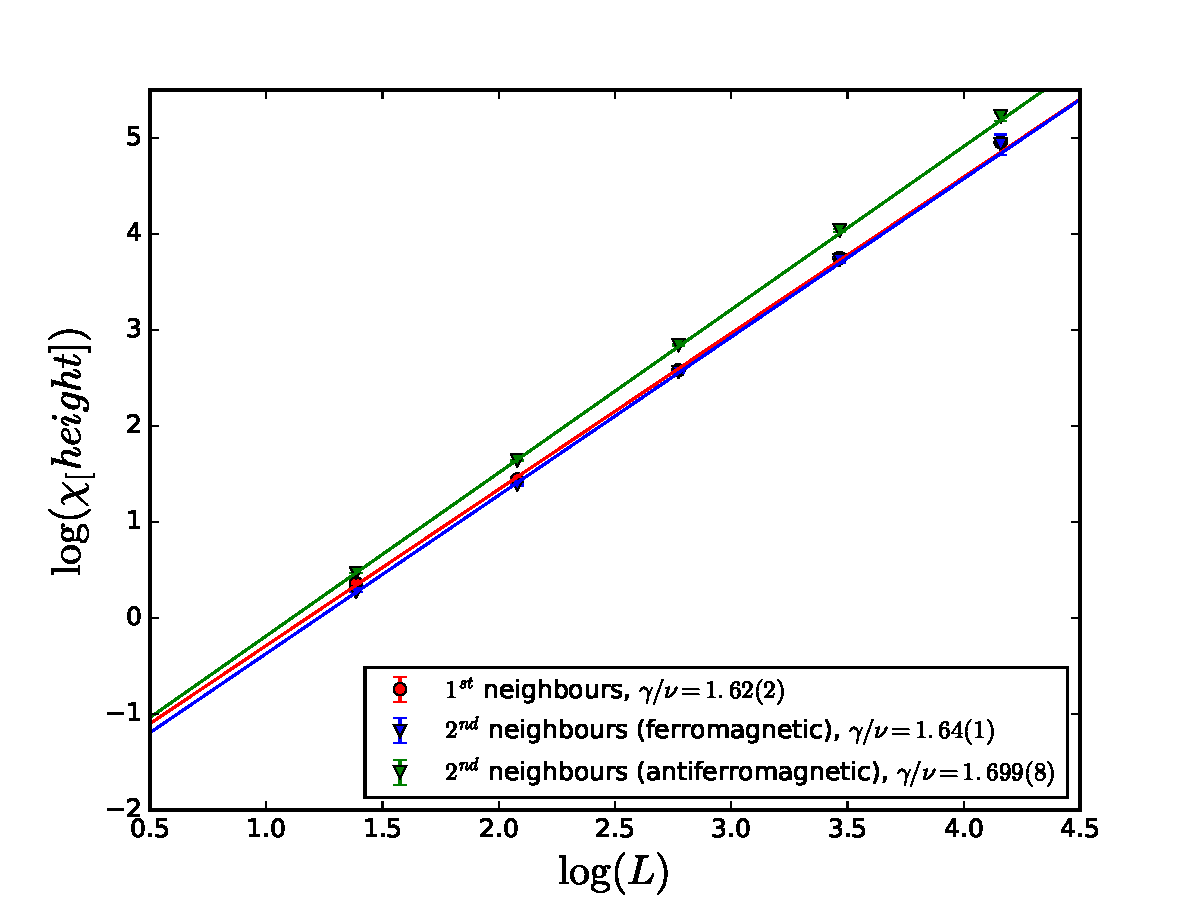
\includegraphics[width=\textwidth]{images/plot_height.pdf}
    \caption{Height}
    \label{scaling_height}
  \end{subfigure}
  \begin{subfigure}[b]{0.32\textwidth}
    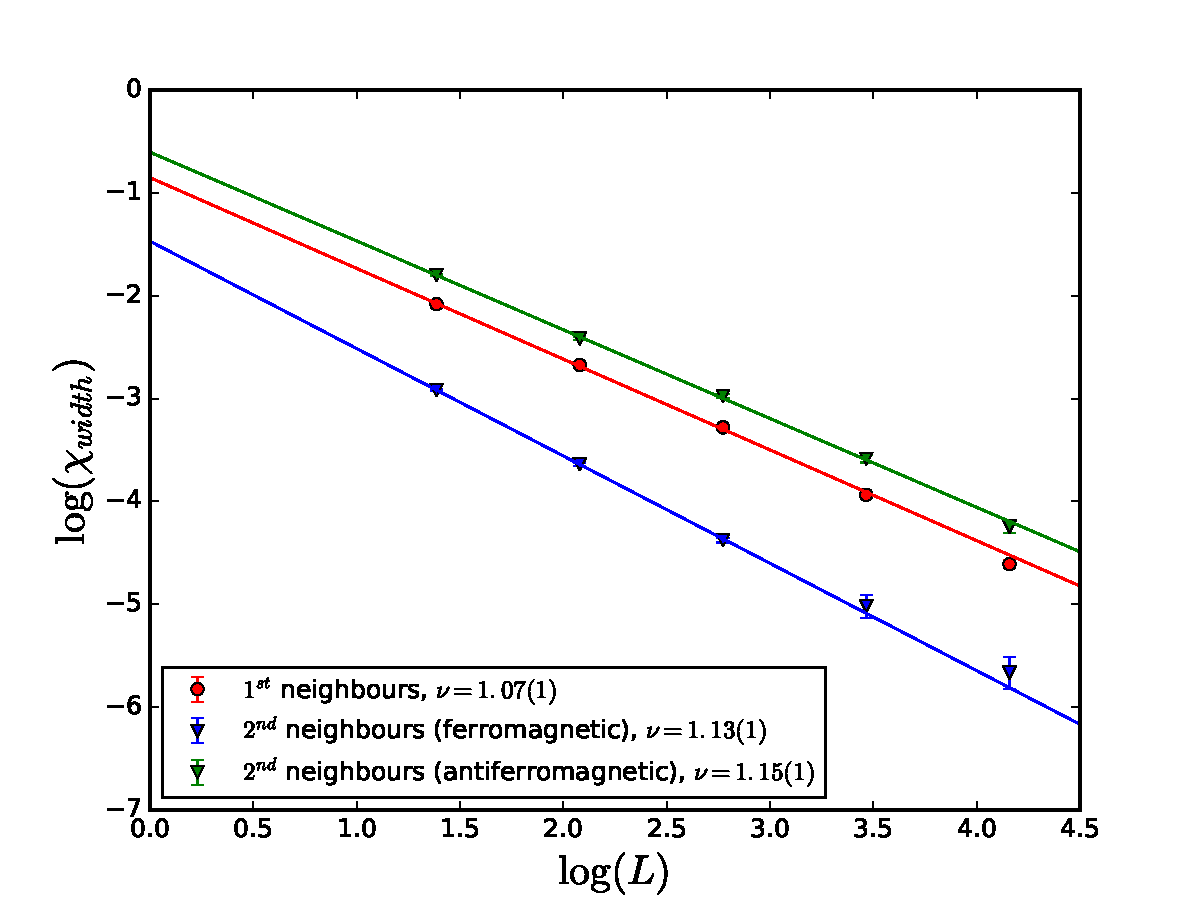
\includegraphics[width=\textwidth]{images/plot_width.pdf}
    \caption{Width}
    \label{scaling_width}
  \end{subfigure}
    \begin{subfigure}[b]{0.32\textwidth}
    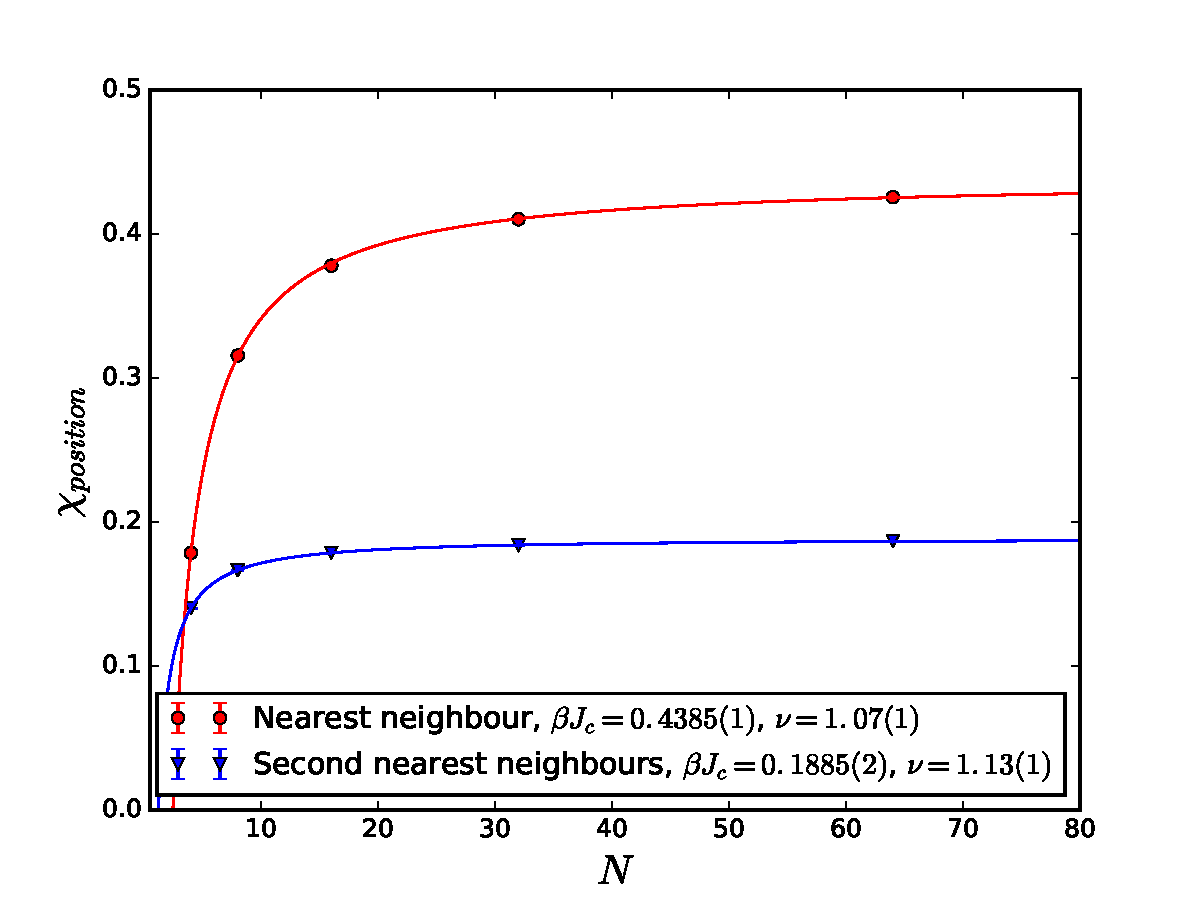
\includegraphics[width=\textwidth]{images/plot_pos.pdf}
    \caption{Positions}
    \label{scaling_pos}
  \end{subfigure}
  \caption{Scaling behaviour .}
  \label{scaling}
\end{figure*}

As a system approaches a critical phase transition, the behaviour of its physical quantities is described by power laws. The exponents corresponding to these power laws are called the \emph{critical exponents}. For the Ising model we can write:

\begin{align}
&\chi \sim |T-T_c|^{-\gamma} \\
& C_v \sim |T-T_c|^{-\alpha} \\
& \xi \sim |T-T_c|^{-\nu} \\
& m \sim |T-T_c|^{\beta}
\end{align}

The exact values for the critical exponents are given by:
\begin{align}
&\gamma = \frac{7}{4} \\
&\alpha = 0 \\
&\nu = 1\\
&\beta = \frac{1}{2} 
\end{align}

\noindent These exponents are said to be \emph{universal} due to the fact that they remain invariant changes in the Hamiltonian that do not affect the system size or its order. Systems governed by different Hamiltonians but with the same critical exponents are said to belong to the same \emph{universality class}. 

It is important to note that analytical exponents are actually obtained by taking the system size $LxL$ to be infinite. The thermodynamic quantities will be smooth functions of temperature for a finite system, which means that we will not see a divergence at the critical point, but a smooth peak. As we increase the system size we observe that height, width and position of this peak change according to a set of equations, called \emph{scaling laws}. Suppose we have a thermodynamic quantity $A$ with critical exponent $\sigma$ (i.e. $A \sim |T-T_c|^{-\sigma}$ close to $T_c$): it can be shown that the peak height of $A$ as a function of $T$ (or $\beta J$, in our case) scales as $L^{\sigma/\nu}$, while its position and width scale as $L^{-\nu}$.

These three quantities were tracked for the magnetic susceptibility $\chi$ for different values of $L$ by fitting the peaks to a Gaussian function. Besides the system described by \eqref{ising_hamiltonian}, we considered two other Hamiltonians:

\begin{align}
\label{second_neigh_hamil}
H_2 = -J\sum_{\mean{ij}} s_i s_j  -J\sum_{\mean{\mean{ij}}} s_i s_j \\
\label{anti_hamil}
H_3 = -J\sum_{\mean{ij}} s_i s_j + 0.3 J \sum_{\mean{\mean{ij}}} s_i s_j 
\end{align}

\noindent where $\sum_{\mean{ij}}$ and $\sum_{\mean{\mean{ij}}}$ denote sums over first and second neighbours respectively and $J$ is taken to be positive. These two equation take into account the interaction with second neighbours: in equation~\ref{second_neigh_hamil}, the added contribution is ferromagnetic, while the second neighbour interaction in equation~\ref{anti_hamil} is weakly anti-ferromagnetic.

The results obtained for the critical exponents through finite-size scaling are shown in Figure \ref{scaling} and reported in Table 1. The critical exponents were found to be very close to the exact results for the 2D Ising model ($\frac{\gamma}{\nu} = 1.75$, $\nu = 1$). Furthermore one also sees that although both systems exhibit different critical temperatures the critical exponents are very similar, indicating that both systems belong to the same universality class.

\noindent \addvbuffer[12pt 8pt]{\resizebox{\columnwidth}{!}{
\begin{tabular}{ccccc}
Interaction order & $\beta J_c$ & $\nu \left(\chi_{height}\right)$ & $\nu \left(\chi_{position}\right)$ & $\gamma/\nu$ \\
\hline
$1^{st}$ & 0.4385(1) & 1.07(1) & 1.07(1) & 1.62(2)  \\
$2^{nd} (ferromagnetic)$ & 0.1885(2) & 1.13(1) & 1.13(1) & 1.64(1)   \\
$2^{nd} (antiferromagnetic)$& 0.7382(8) & 1.15(1) & 1.12(1) & 1.699(8) 
\end{tabular}}}

One can also study the behaviour the magnetization at $T_c$ which is expected to satisfy the following scaling relation \cite{tang}:
\begin{equation}
m(T_c) \propto L^{\beta/\nu}
\end{equation}

In figure \ref{scaling_magnetization} the magnetization at the critical temperature is plotted as function of the system size for a system with nearest neighbour ferromagnetic interactions (Hamiltonian in \eqref{ising_hamiltonian}) \footnote{Next nearest neighbour interactions were not considered due to the fact that they were implemented using the Metropolis algorithm, which suffers from critical slowing down. As such, it is computationally very taxing to obtain good estimates for $m(T_c)$.}. The critical exponent obtained from the slope of the line $\beta = 0.115(3)$ is close to the exact value of $\beta = 0.125$.

\begin{figure}[H]
\centering
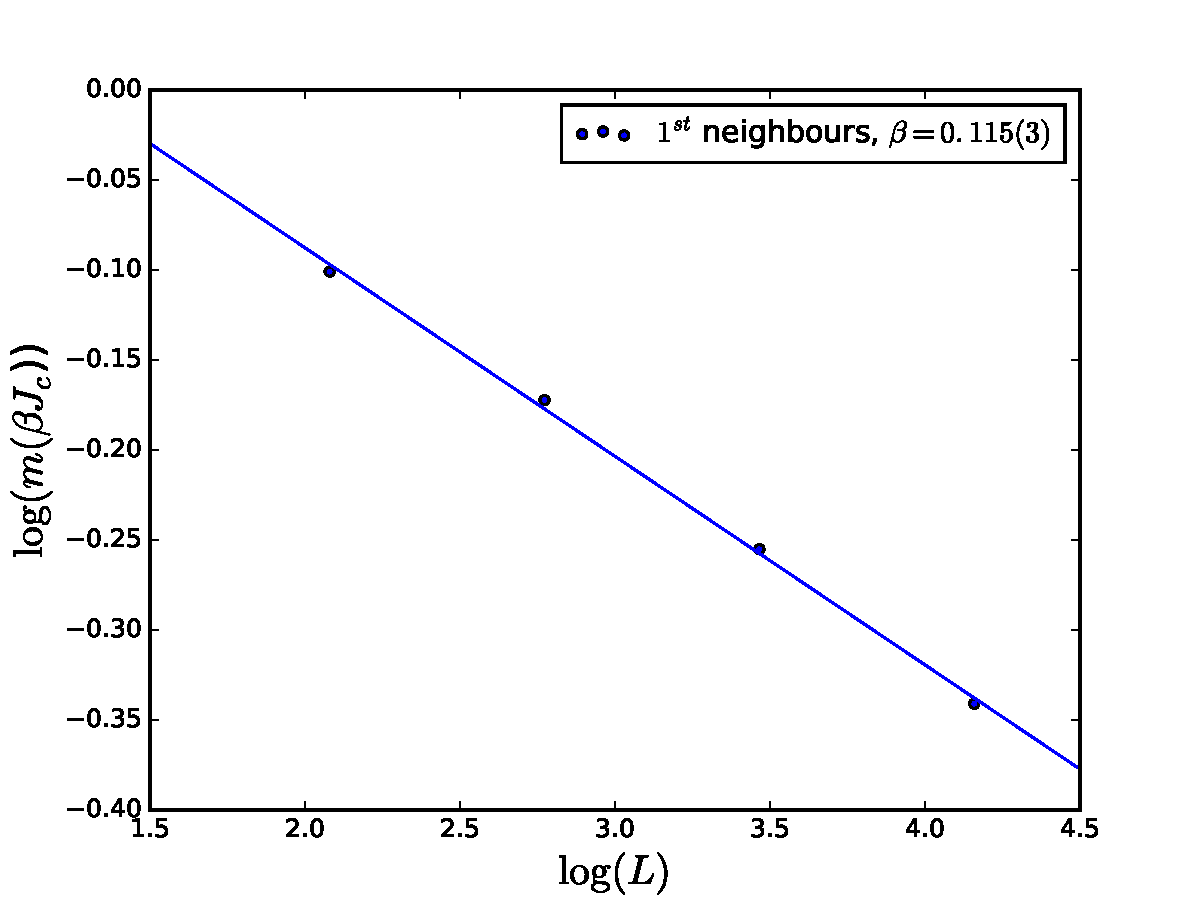
\includegraphics[scale=0.4]{images/plot_magnetization.pdf}
\caption{Scaling behaviour of the magnetization at the critical temperature $m(T_c)$.}
\label{scaling_magnetization}
\end{figure}

\subsection{XY Model}
The XY model undergoes a phase transition (known as the Kosterlitz-Thouless transition) from bound vortex-antivortex pairs at low temperatures to unpaired vortices and anti-vortices. 

The helicity modulus $\Gamma$ (helicity modulus) quantifies the free energy needed to 'twist' the spins and can be expressed as:

\begin{align}
\Gamma &= \frac{J}{2L^2}\left\{ \mean{\sum_{\mean{ij}} \cos(\theta_i - \theta_j)} - \frac{J}{k_B T} \mean{\left[ \sum_i \sin( \theta_i - \theta_{i+ \vec{e_x}}) \right]^2}\right.\nonumber \\
 &\qquad \left. {}  - \frac{J}{k_B T} \mean{\left[ \sum_i \sin( \theta_i - \theta_{i+ \vec{e_y}}) \right]^2} \right\}
\end{align}

For infinite systems $\Gamma$ drops to zero at the KT critical temperature $T_{KT}$. It can be shown \cite{thijssen} that  $\Gamma$ has a universal value of $2k_B T_{KT}/\pi$ at the KT transition.

$\Gamma/J$ is plotted in figure \ref{helicity_modulus_fig} as a function of temperature. The line $ \Gamma/J = 2k_B T/(J \pi)$ is also shown in order to determine $T_{KT}$.

\begin{figure}[H]
\centering
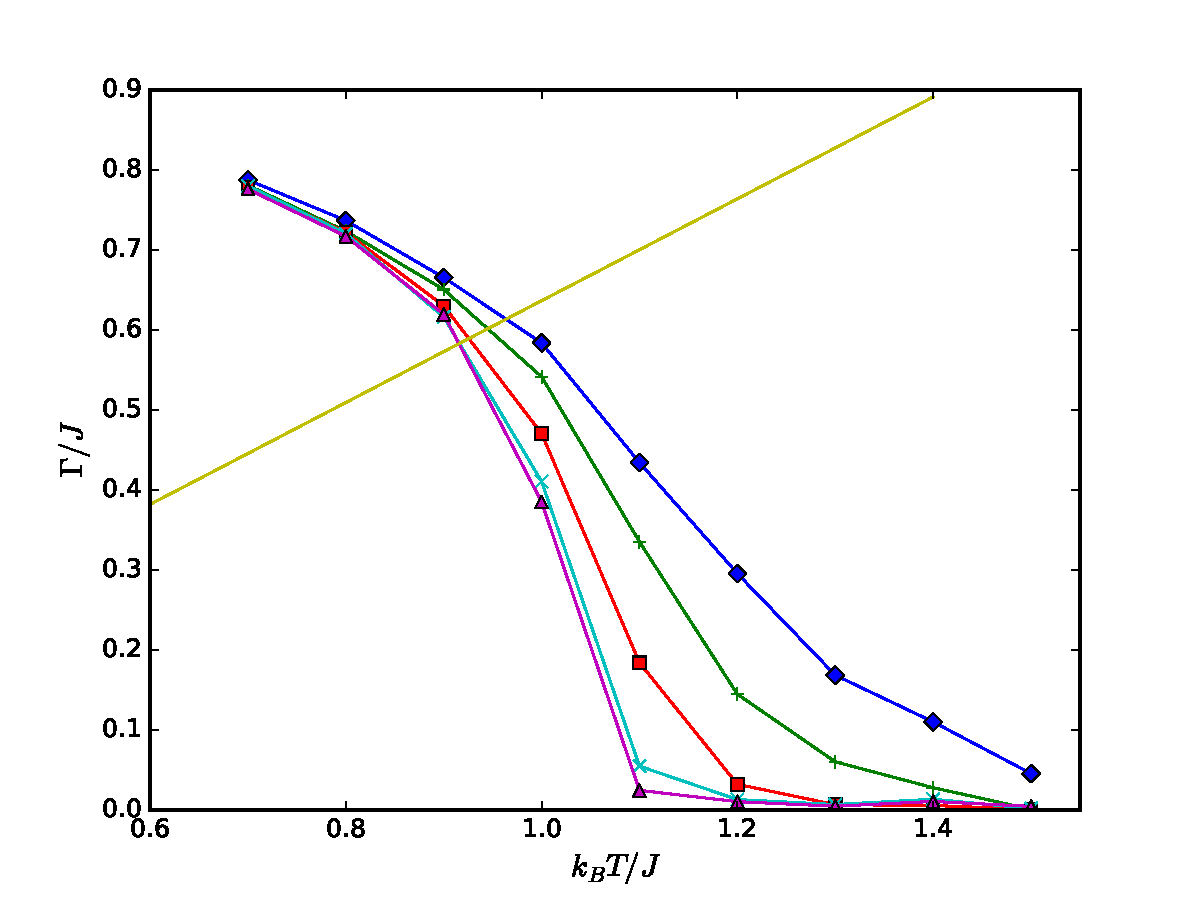
\includegraphics[scale=0.4]{images/helicity_modulus.pdf}
\caption{The helicity modulus in units of the coupling constant J of the XY model vs. the inverse coupling constant in units of $k_B T$. The intersection with the straight line gives the critical temperature $T_{KT}$.}
\label{helicity_modulus_fig}
\end{figure}

The results are similar to those obtained by Thijssen \cite{thijssen}. We can note that, as the system size increases, the slope of the curves becomes steeper and its behaviour becomes non-analytic close to the critical temperature.

By checking the intersection of the line with the results $L=100$ we can obtain a rough estimate for critical temperature. We find $\beta_{KT} \approx 1.121$ which is very close to the value of $\beta_{KT} \approx 1.120(1)$ reported in \cite{dukovski}.

%------------------------------------------------
\section{Conclusion}
In this paper, we presented the results obtained through the Monte Carlo simulation of the Ising model and the XY Model.
The behaviour of the magnetization, susceptibility, binder cumulant and specific heat was found thanks to the Hoshen-Kopelman algorithm and resembles closely the theoretical prediction. Using finite-size scaling, we were able to calculate some of the critical exponent, obtaining accurate values for all the interaction orders we considered and consequently proving their universality.
In the simulation of the XY model, we found an estimate for the helicity modulus, showing how the Monte Carlo algorithms can be used to predict the behaviour of a variety of physical systems with reasonable accuracy.
%----------------------------------------------------------------------------------------
%	REFERENCE LIST
%----------------------------------------------------------------------------------------

\begin{thebibliography}{99} % Bibliography - this is intentionally simple in this template

\bibitem{thijssen}
J.M.Thijssen,
\newblock {\em Computational Physics}, Cambridge University Press, 2nd Edition, 2007.

\bibitem{joas}
C. Joas, 
\newblock {\em Introduction to the Hoshen-Kopelman algorithm and its application to nodal domain statistics}, Online Lecture notes, (\verb+https://webhome.weizmann.ac.il/home/feamit/+ \\ \verb+nodalweek/c_joas_nodalweek.pdf+)
\bibitem{lecture_notes}
K. Rummukainen,
\newblock {\em Simulation methods in physics}, Online Lecture notes (\verb+http://www.helsinki.fi/~rummukai/simu/+)

\bibitem{tang}
S. Tang and D. P. Landau
{\em Monte Carlo study of dynamic universality in two-dimensional Potts models}, Phys. Rev. B, 36, 567–73, 1985

\bibitem{dukovski}
I. Dukovski, J. Machta, and L. V. Chayes, 
\newblock {\em Invaded cluster simulations of the XY model in two and three dimensions}, Phys. Rev. E, 65, 026702, 2002.
\end{thebibliography}

%----------------------------------------------------------------------------------------
\end{multicols}

\end{document}
 
